\documentclass[11pt,a4paper]{article}

\usepackage{amsmath} %for mathemathic formulas
\usepackage{amssymb}
\usepackage[ngerman]{babel} %for the german language by the spellling reform (without the package the date would look like April 20, 2020)
\usepackage{enumitem} %for enumeration surrounding 
\usepackage{graphicx} %for pictures
\usepackage{siunitx}
\usepackage{float}

\title{Blatt 11}
\date{\today}
\author{Hannah Rotgeri \and Feline Heinzelmann}

\begin{document}
    \maketitle

    \section*{Aufgabe 1}
	\begin{itemize}
		\item[a)] 
			Transversale Instabilitäten führen zu einer Modulation in der Signalhöhe mit Auswirkung auf das Energieintervall (bei Zunahme verringert sich Brillanz).
			Longitudinale Instabilitäten führen dagegen zu einer variierenden Ankunftszeit an der Elektrode, wodurch die Zahl der auftreffenden Photonen pro Zeiteinheit varriiert. 
			Die Brillanz ist damit zeiltich instabil und kann zeitweise deutlich vermindert sein. 
			Schwingungen in transversaler und longitudinaler Richutng destabilisieren insgesamt die Brillanz. \newline
			Korrektur: Transversale Instabilitäten vergrößern den Strahlquerschnitt und die Strahldivergenz, longitudinale Instabilitäten die mittlere Paketlänge und die Energiebreite.

		\item[b)]
			Dämpfungen der longitudinalen Schwingungen der Teilchenpakete beeinflussen die Ankunftzeit der Elektronen. Um die Elektronen zu verzögern oder zu beschleunigen, gibt es zwei Möglichkeiten: Ihren Ort oder ihre Energie ändern. Messen kann longitudinal ihre Ankunftszeit oder die Energiebreite.
			Allerdings kann man nur das letztere aktiv beeinflussen, und zwar mithilfe eines Hohlraumresonators. Aufgrund der sehr langsamen Synchrotron-Oszillation, die das Elektronenpaket ausführt, muss man mit der Dämpfung durch den Hohlraumresonator warten bis sich das Teilchen energetisch 
			zu einer günstigen Energieabweichung verschoben ist und kickt optimatimalerweise die Elektronen beim Punkt $z=0$. Der Hohlraumresonator fungiert als longitudinaler Kicker.
			\begin{figure}
				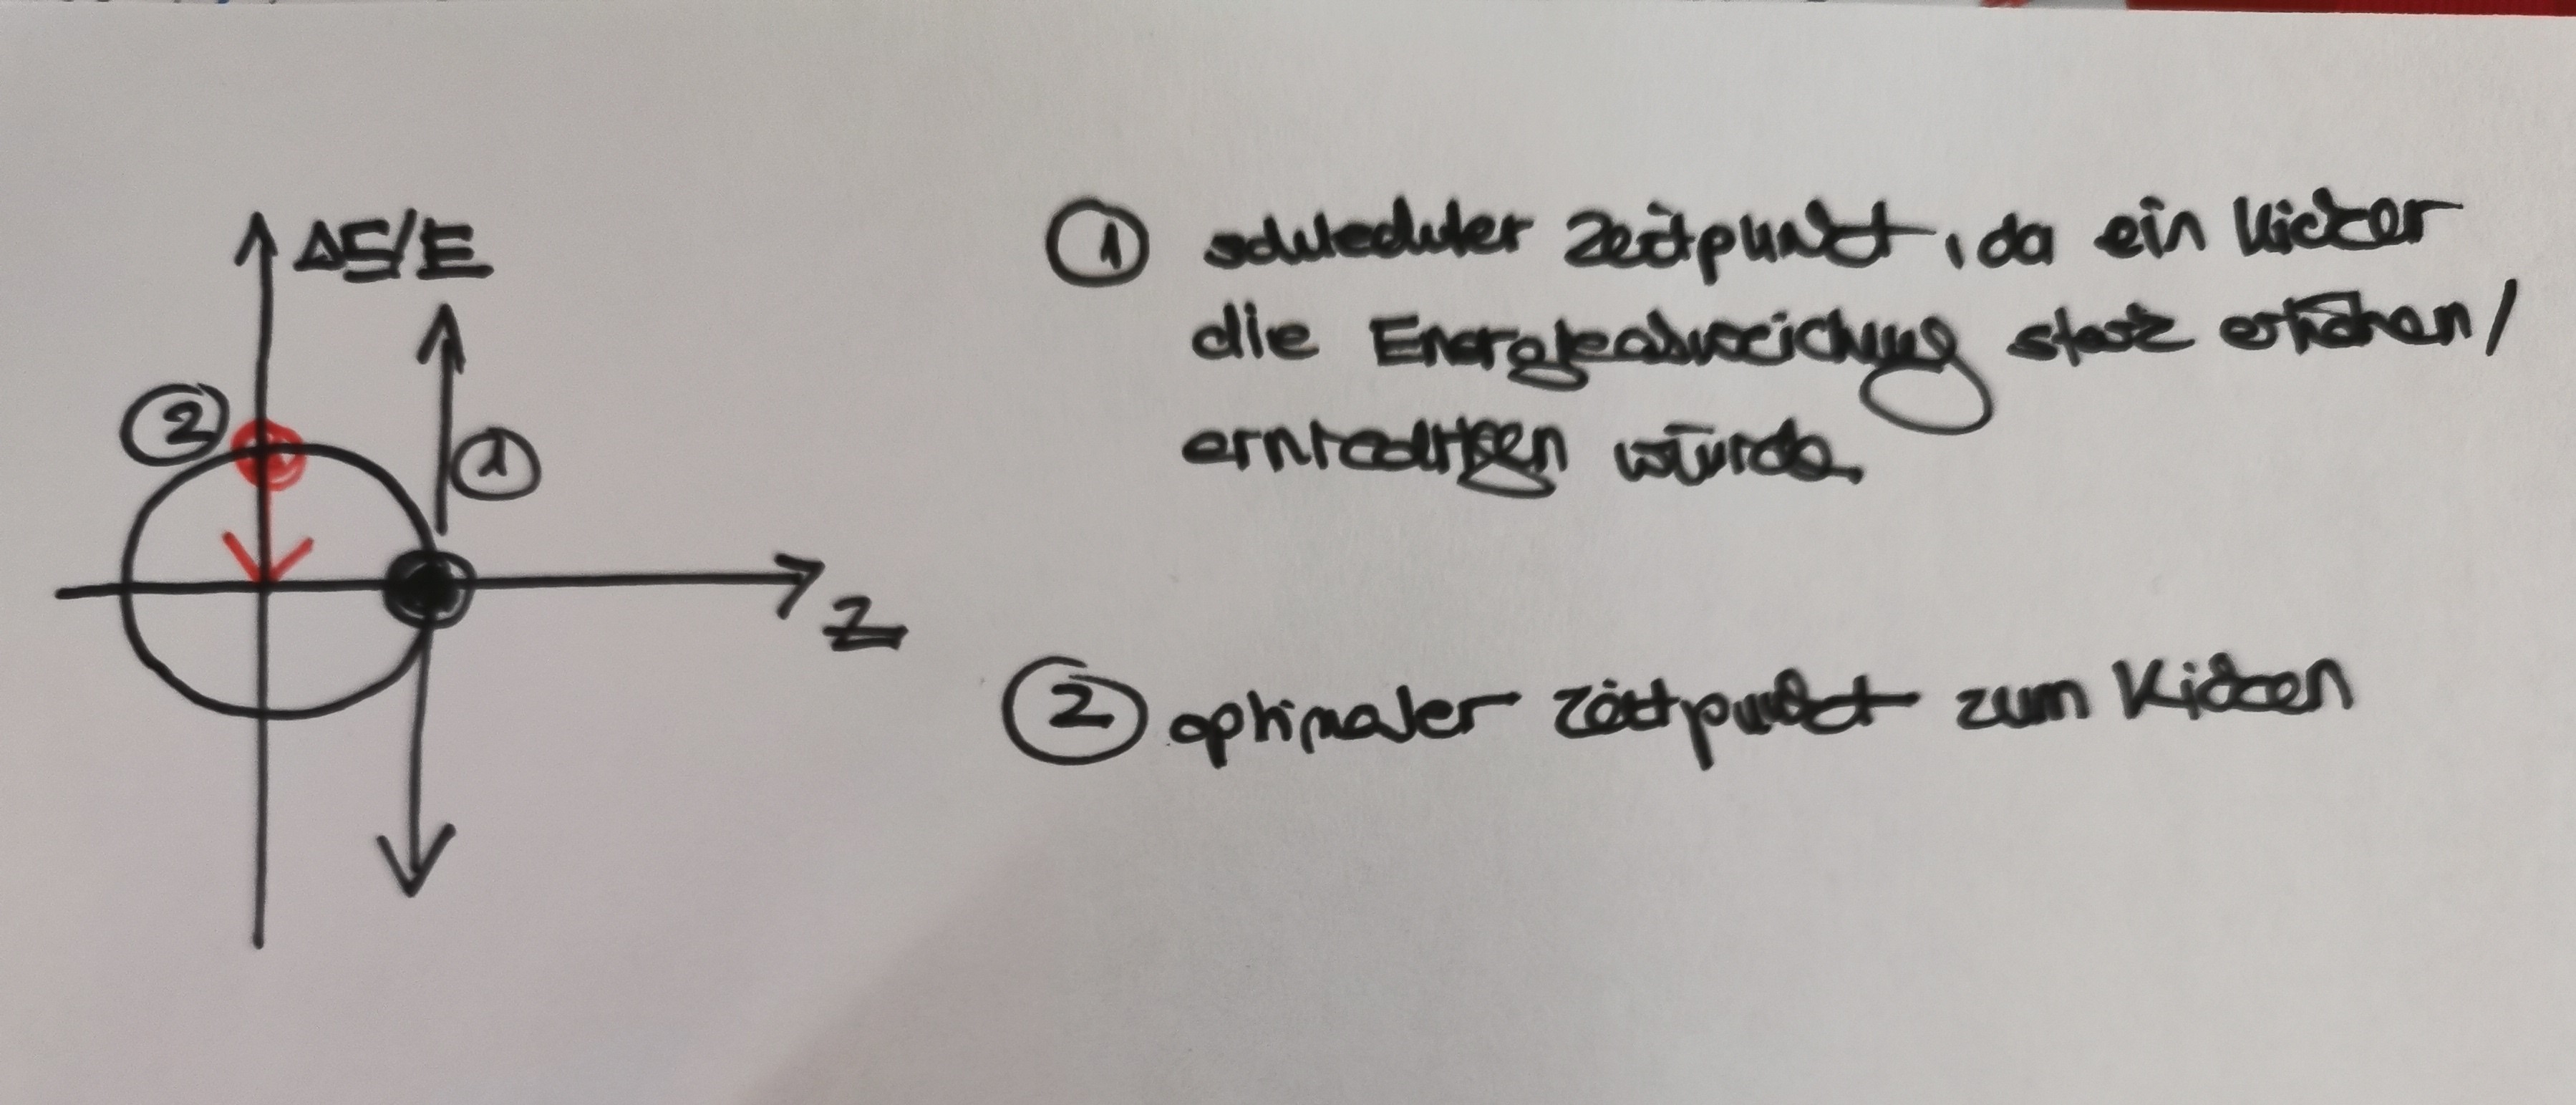
\includegraphics[width=0.5\textwidth]{IMG_20200708_085910.jpg}
			\end{figure}

	\end{itemize}


	
    \section*{Aufgabe 2}
	\begin{itemize}
		\item[a)] 
			Gegeben: $U = \SI{115.2}{m}$, $f_{HF} = \SI{500}{MHz}$ \newline
			Gesucht: Anzahl der Eigenmoden für longitudinale und transverale Schwingungsmoden \newline
			Sowohl bei den transversalen als auch bei den longitudinalen Schwingungen der Teilchenpakete existieren bei gekoppelten Teilchenpaketen h Eigenmoden, 
			die sich als Seitenbänder um bestimmte Umlauf-Harmonische zeigen. $h$ ergibt sich aus:
			\begin{align*}
				h = \frac{\omega_{HF}}{\omega_0} = \frac{2\pi \cdot f_{HF}}{2\pi \cdot f_{0}} \\
				\text{mit} \, f_0 = 1/T = c/U = \SI{2.6}{MHz}\\
				h = 192 \\
			\end{align*}
			Damit ergeben sich 192 Eigenmoden.
		\item[b)]
			Gegeben: $f_{HF} = \SI{499.82}{MHz}$, $(\frac{\omega_{\beta}}{\omega_0})_{1} = 9.21$, \newline
			$(\frac{\omega_{\beta}}{\omega_0})_{2} = 3.36$, $f_{0} = \SI{15}{kHz}$  \newline
			Die Betatronfrequenz ist der franktionierte Arbeitspunktanteil und ist kleiner als die Umlauffrequenz.
			Mit $f_s$ als Synchrotronband und $f_Q$ als Betatronseitenband.
			$1/\tau$ ist die Dämpfungsrate mit $\tau$ als Dämpfungszeit.
 	\end{itemize}

	\section*{Aufgabe 3}

		Die Größenordung der Anstiegsrate scheint nicht zu passen. Theoretisch wäre der Strahl stabil, 
		wenn die Anstiegsrate geringer ist als die Dämpfung, die angegeben ist.
		Die angegebene Dämpfung entspricht aber einer Rate in der Größenordung $10³$.
		Die berechnete Anstiegsrate entspricht $10¹⁷$.
		Daher lässt sich auch in der b) nicht der gesuchte Radius bestimmen.
		Es zeigt sich, dass bei kleinerem Radius die Rate höher wird.

		\noindent Korrigiert:
		\begin{figure}
			\includegraphics[width=\textwidth]{build/Arbeitspunkt.pdf}
		\end{figure}

\end{document}
